\chapter {Interfacing a Thermistor}
\thispagestyle{empty}
\label{thermistor}

\newcommand{\LocTHERMfig}{\Origin/user-code/thermistor/figures}
\newcommand{\LocTHERMscicode}{\Origin/user-code/thermistor/scilab}
\newcommand{\LocTHERMscibrief}[1]{{\tt \seqsplit{%
Origin/user-code/thermistor/scilab/#1}}, see \fnrefp{fn:file-loc}}
\newcommand{\LocTHERMardcode}{\Origin/user-code/thermistor/arduino}
\newcommand{\LocTHERMardbrief}[1]{{\tt \seqsplit{%
Origin/user-code/thermistor/arduino/#1}}, see \fnrefp{fn:file-loc}}

%%%%%%%%%%%python starts
\newcommand{\LocTHERMpycode}{\Origin/user-code/thermistor/python}
\newcommand{\LocTHERMpybrief}[1]{{\tt \seqsplit{%
Origin/user-code/thermistor/python/#1}}, see \fnrefp{fn:file-loc}}
%%%%%%%%%%%python ends

%%%%%%%%%julia
\newcommand{\LocTHERMjuliacode}{\Origin/user-code/thermistor/julia}
\newcommand{\LocTHERMjuliabrief}[1]{{\tt \seqsplit{%
    Origin/user-code/thermistor/julia/#1}}, see \fnrefp{fn:file-loc}}
%%%%%%julia

%%%%%%%%%OpenModelica starts
\newcommand{\LocTHERMOpenModelicacode}{\Origin/user-code/thermistor/OpenModelica}
\newcommand{\LocTHERMOpenModelicabrief}[1]{{\tt \seqsplit{%
    Origin/user-code/thermistor/OpenModelica/#1}}, see \fnrefp{fn:file-loc}}
%%%%%%OpenModelica ends

A thermistor, usually made of semiconductors or metallic oxides, is a
temperature dependent/sensitive resistor. Depending on the temperature
in the vicinity of the thermistor, its resistance changes. Thermistors
are available in two types, NTC and PTC. NTC stands for Negative
Temperature Coefficient and PTC for Positive Temperature
Coefficient. In NTC thermistors, the resistance decreases with the
increase in temperature and vice versa. Whereas, for PTC types, the
resistance increases with an increase in temperature and vice
versa. The temperature ranges, typically, from $-55^{\circ}$ Celsius
to $+125^{\circ}$ Celsius.  

Thermistors are available in a variety of shapes such as beads, rods,
flakes, and discs. Due to their compact size and low cost, they are
widely used in the applications where even imprecise temperature
sensing is sufficient. They, however, suffer from noise and hence need
noise compensation. In this chapter we shall interface a thermistor
with the \arduino\ board.

\section{Preliminaries}
A typical thermistor and its symbolic representation are shown in
\ref{fig:therm} and \ref{fig:thermsym} respectively. The thermistor is
available on the shield provided with the kit.  It is a bead type
thermistor having a resistance of 10k at room temperature. A voltage
divider network is formed using thermistor and another fixed 10k
resistor. A voltage of 5 volts is applied across the series
combination of the thermistor and the fixed 10k resistor. Voltage
across the fixed resistor is sensed and is given to the ADC via pin
4. Hence at room temperature, both the resistors offer 10k resistance
resulting in dividing the 5V equally. A buzzer is also connected on
pin 3 which is a digital output pin.
Connections for this experiment are shown in \ref{fig:therm-conn}
and \ref{fig:buzzer-conn}.  Nevertheless, the user doesn't need to
connect any wire or component explicitly.


\begin{figure}
\centering
\subfloat[Pictorial representation of a thermistor\cite{therm-wiki}]{
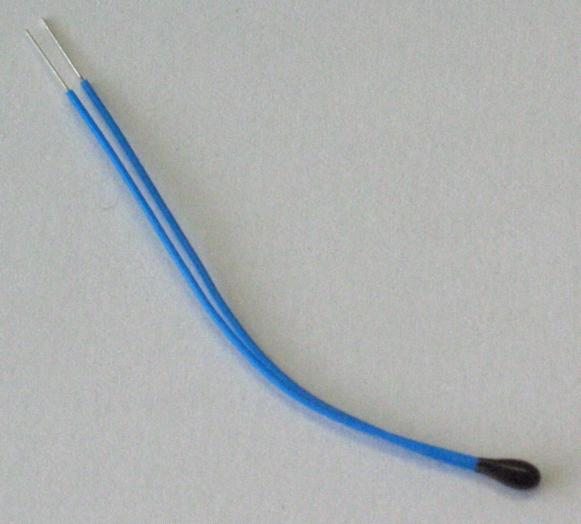
\includegraphics[width=\smfig]{\LocTHERMfig/NTC-bead.jpg}
\label{fig:therm}} \hfill
\subfloat[Symbolic representation of a thermistor]{

\includegraphics[width=\tnfig]{\LocTHERMfig/therm-sym.png}
\label{fig:thermsym}}
\caption{Pictorial and symbolic representation of a thermistor}
\end{figure}


\begin{figure}
\centering
\subfloat[Thermistor connection diagram]{
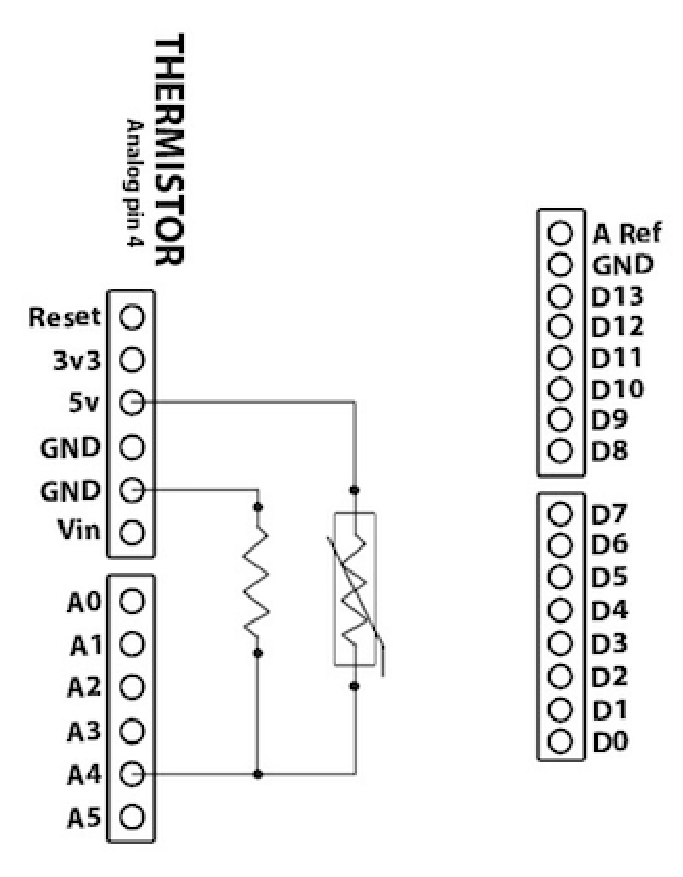
\includegraphics[width=\smfig]
{\LocTHERMfig/THERMISTOR-Diagram-crop.pdf} 
\label{fig:therm-conn}} \hfill
\subfloat[Buzzer connection diagram]{
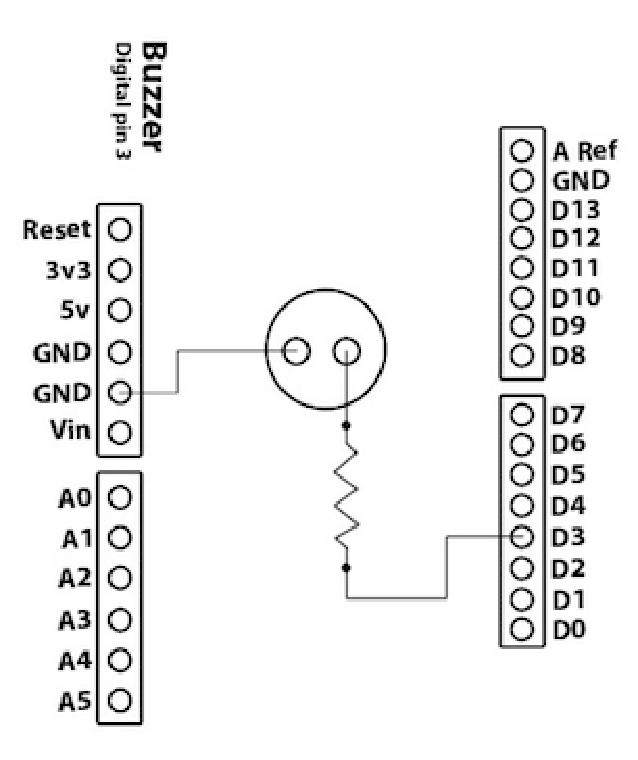
\includegraphics[width=\smfig]
{\LocTHERMfig/BUZZER-Diagram-crop.pdf} 
\label{fig:buzzer-conn}}
\caption{Thermistor and buzzer connection diagrams}
\end{figure}

\section{Connecting a thermistor with \arduino\ using a breadboard}
This section is useful for those who either don't have a shield or don't want to use the shield
for performing the experiments given in this chapter. 

A breadboard is a device for holding the components of a circuit and connecting 
them together. We can build an electronic circuit on a breadboard without doing any 
soldering. To know more about the breadboard and other electronic components, 
one should watch the Spoken Tutorials on Arduino as published on
{\tt https://spoken-tutorial.org/}. Ideally, one should go through all the
tutorials labeled as Basic. However, we strongly recommend the readers should
watch the fifth and sixth tutorials, i.e., First Arduino Program and 
Arduino with Tricolor LED and Push button.

In case you have a thermistor, and you want to connect it with \arduino\ on a breadboard, 
please refer to \figref{fig:ard-therm-bread}. The connections given in this figure 
can be used to read values from the thermistor connected to analog pin 4 on \arduino\
board. 
\begin{figure}
  \centering
  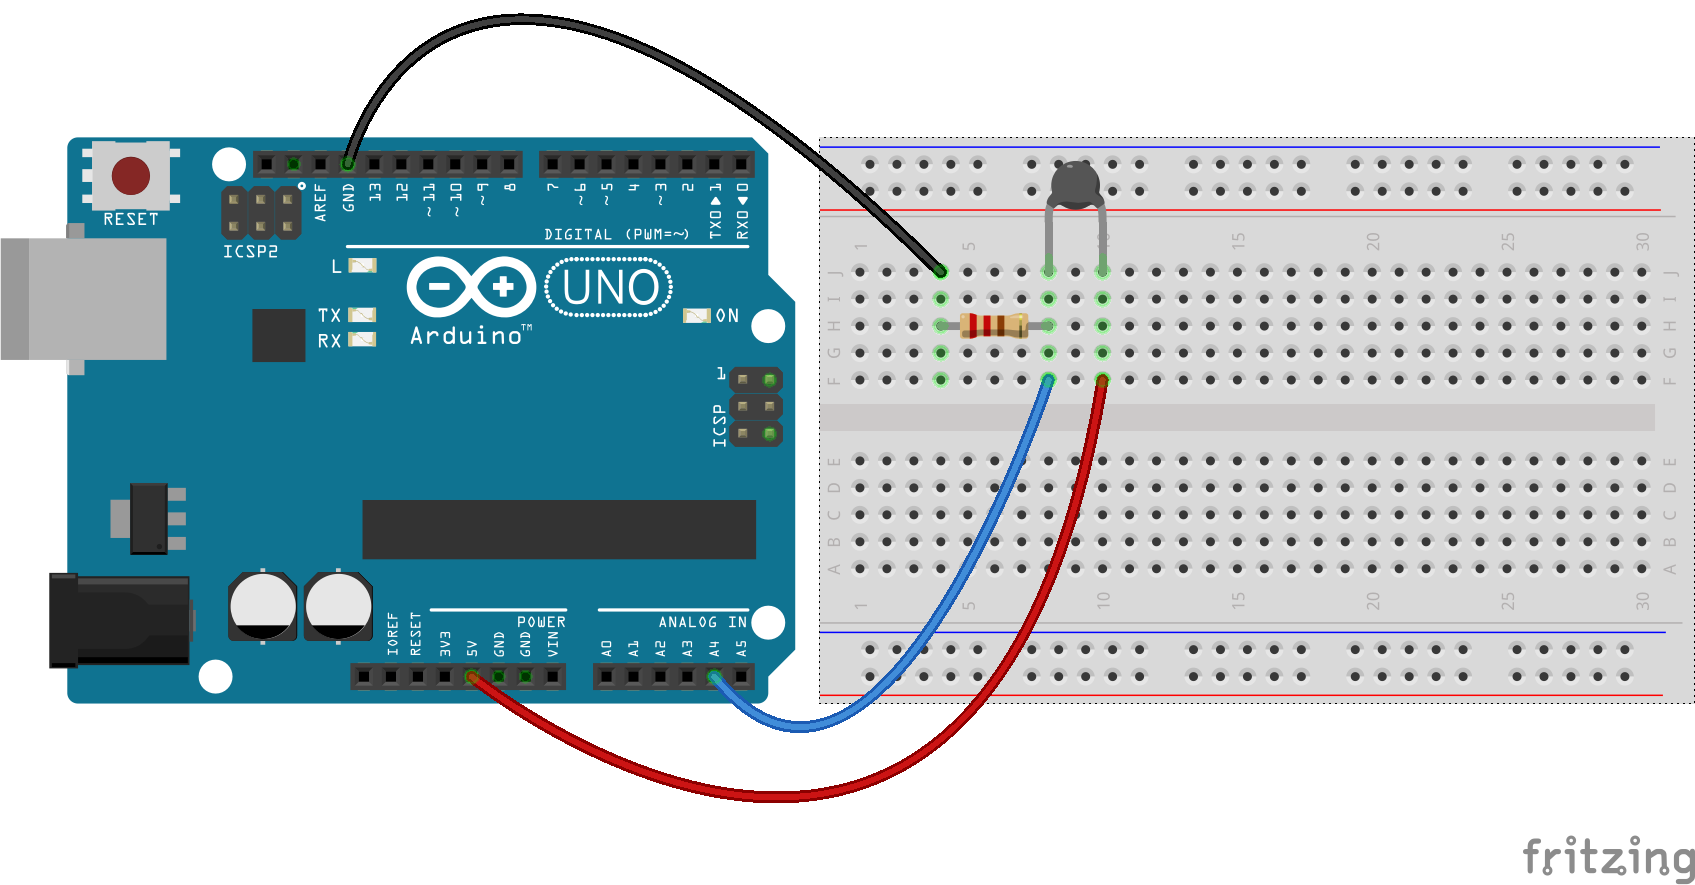
\includegraphics[width=\textwidth]{\LocTHERMfig/thermistor.png}
  \caption{A thermistor to read its values with Arduino Uno using a breadboard}
  %\redcolor{connected on pin no. D12}}
  \label{fig:ard-therm-bread}
\end{figure}
As shown in \figref{fig:ard-therm-bread}, one leg of the thermistor is connected 
to 5V on \arduino\ and the other leg to the analog pin 4 on  \arduino. A resistor is also 
connected to the same leg and grounded. From \figref{fig:therm-conn} and \figref{fig:ard-therm-bread}, one can infer that a resistor 
along with the thermistor is used to create a voltage divider circuit. The varying 
resistance of the thermistor is converted to a varying voltage. Finally, this voltage is used 
by the analog pin 4 of \arduino\ in its logic. 

\begin{figure}
  \centering
  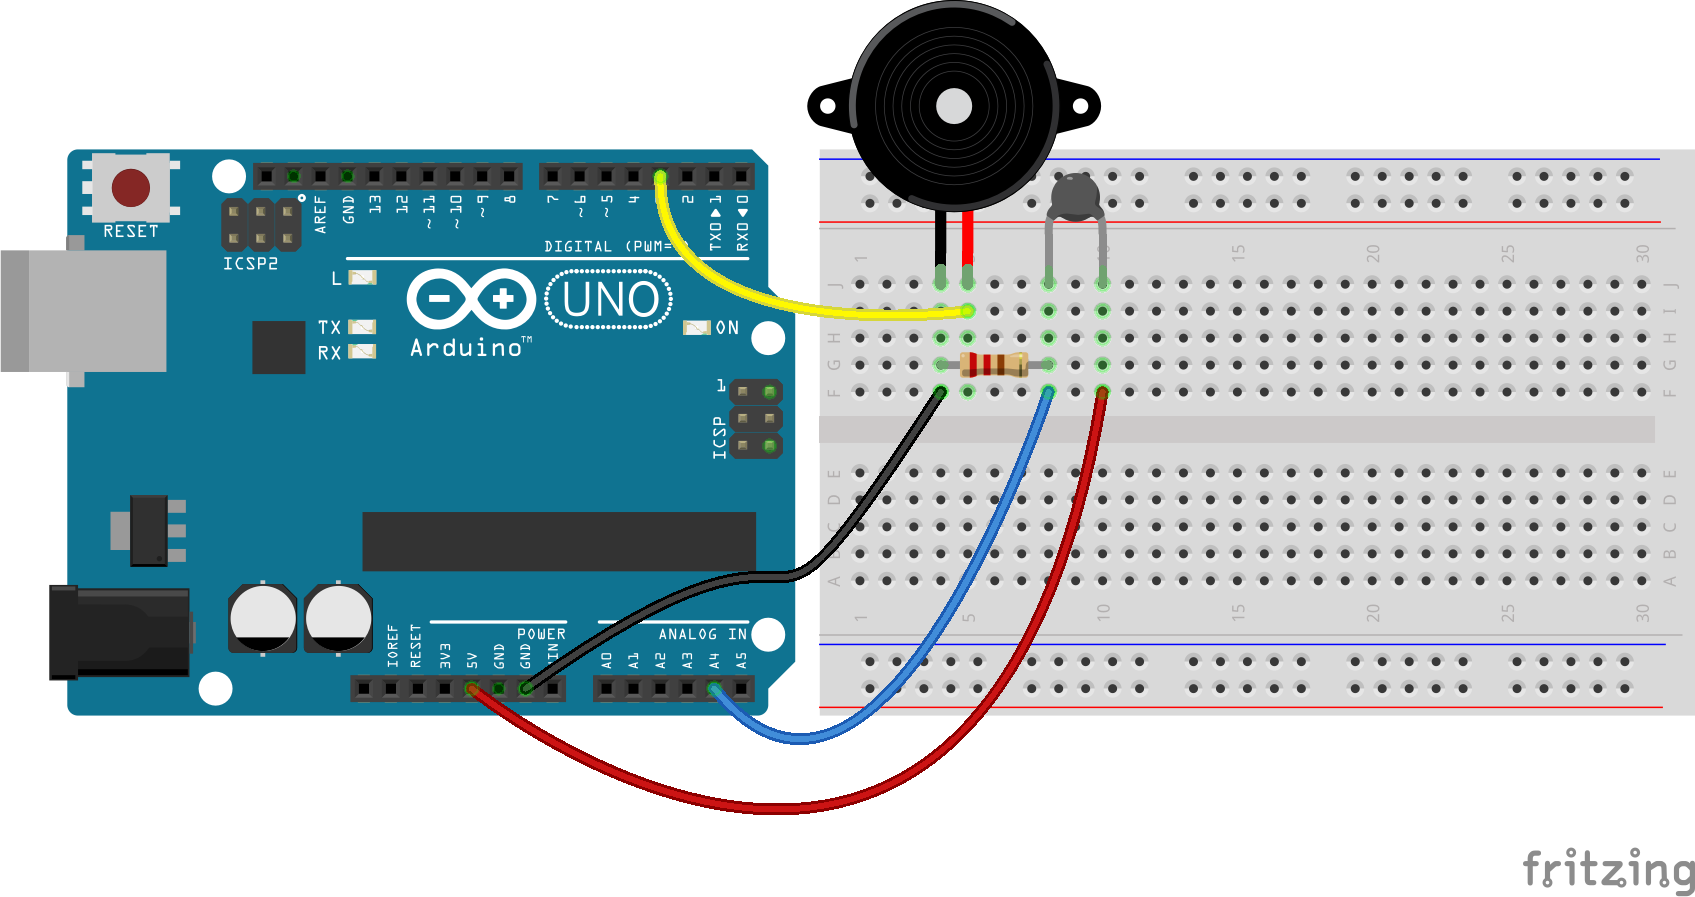
\includegraphics[width=\textwidth]{\LocTHERMfig/thermistor-buzzer.png}
  \caption{A thermistor to control a buzzer with Arduino Uno using a breadboard}
  %\redcolor{connected on pin no. D12}}
  \label{fig:ard-therm-buzzer}
\end{figure}
The connections shown in \figref{fig:ard-therm-buzzer} can be used to control a buzzer, 
depending on the values from the thermistor. As shown in \figref{fig:ard-therm-buzzer}, 
digital pin 3 on \arduino\ is connected to the one of the legs of the buzzer. Another 
leg of the buzzer is connected to GND of \arduino.    


\section{Interfacing the Thermistor from the Arduino IDE}
\subsection{Interfacing the Thermistor}
In this section we will learn how to read values from the thermistor
connected at pin 4 of the \arduino\ board. We shall also see how to
drive a buzzer depending upon the thermistor values.

\begin{enumerate}
\item A simple code to read the values from thermistor is given in \ardref{ard:therm-read}. The arduino IDE based command for the analog read functionality is given by.
\lstinputlisting[firstline=9,lastline=9]  {\LocTHERMardcode/therm-read/therm-read.ino} 
where {\tt A4} represents the analog pin 4 to be read. The read value is stored in variable {\tt value} and is displayed using \lstinputlisting[firstline=10,lastline=10]  {\LocTHERMardcode/therm-read/therm-read.ino} 
The command on next line

\lstinputlisting[firstline=11,lastline=11]  {\LocTHERMardcode/therm-read/therm-read.ino} 
 is used to put a delay of 500 milliseconds. This is to avoid very fast display of the read values. The entire reading and display operation is carried out 40 times.

The values can be observed over the serial monitor. The numbers
displayed range from 0 to 1023. At room temperature you may get the
output of ADC around 500. If a heating or cooling source is available,
one can observe the increase or decrease in the ADC output. Although
the thermistor is of NTC type, the ADC output increases with increase
in temperature. This is because the voltage across the fixed resistor
is sensed. 

\item In this experiment, we will turn the buzzer on and off depending
  on the temperature sensed by the thermistor. The program for this is
  available at \ardref{ard:therm-buzzer}. We shall use the ADC output
  to carry this out. The buzzer is connected on pin 3 which is a
  digital output pin. The ADC output value is displayed on the serial
  monitor. At the same time it is compared with value 550. Temperature
  of the thermistor can be raised by just holding it for a
  while. Doing so will transfer heat from the person holding the
  thermistor, thereby raising the temperature of the thermistor. As
  soon as the ADC output exceeds 550, the buzzer is given a digital
  high signal, turning it On. A delay of half a second is introduced
  before the next value is read. This loop is executed 100 times. 
\end{enumerate}

\begin{exercise}
Carry out the following exercise:
\begin{enumerate}
\item Put the thermistor in the vicinity of an Ice bowl. Take care not
  to wet the shield while doing so. Note down the ADC output value for
  0$^{\circ}$Celsius. 
\end{enumerate}
\end{exercise}

\subsection{Arduino Code}
\label{sec:therm-arduino-code}
\addtocontents{ard}{\protect\addvspace{\codclr}}

\begin{ardcode}
  \acaption{Read and display the thermistor values} {Read and display
    the thermistor values.  Available at
    \LocTHERMardbrief{therm-read/therm-read.ino}.}
\label{ard:therm-read}
\lstinputlisting{\LocTHERMardcode/therm-read/therm-read.ino}
\end{ardcode}

\begin{ardcode}
  \acaption{Turning the buzzer on and off using thermistor values}
  {Turning the buzzer on and off using the thermistor values read by
    ADC.  Available at
    \LocTHERMardbrief{therm-buzzer/therm-buzzer.ino}.}
\label{ard:therm-buzzer}
\lstinputlisting{\LocTHERMardcode/therm-buzzer/therm-buzzer.ino}
\end{ardcode}

\section{Interfacing the Thermistor from \scilab}
\subsection{Interfacing the Thermistor}
In this section we will explain a few \scilab\ scripts to read values
from thermistor and to use them.  The {\tt cmd\_analog\_in} command
will be used to read from thermistor connected to an analog input
pin. The experiments will be carried out using \scilab.

\begin{enumerate}
\item In the first experiment, \sciref{sci:therm-read} is used to read
  values from thermistor. First the serial port is opened using the
  command {\tt open\_serial} and passing the correct port number to
  it. The command {\tt cmd\_analog\_in} is used to read from the
  analog pin. The pin number is passed to this command as an
  argument. The read value is stored in some variable. The value is
  then displayed on the scilab console. A sleep of 500 millisecond is
  executed using the {\tt sleep} command and then the reading process
  is repeated 20 times by putting it in a {\tt for} loop. After the
  loop is finished the serial port is closed using the {\tt
    close\_serial} command.

\item In the second experiment, we will use the \scilab\ script to
  turn a buzzer on and off using the thermistor values. The changes in
  the thermistor resistance is sensed as a voltage change between 0 to
  5V. The ADC maps the thermistor voltage readings in to values
  ranging from 0 to 1023. This means 0 for 0 volts and 1023 for 5
  volts. In this experiment we compare the ADC output value with 550
  and as soon as the value exceeds 550 the buzzer is turned on. See
  \sciref{sci:therm-buzzer} for the complete code. We use {\tt if}
  loop to achieve this functionality. Command {\tt cmd\_digital\_out}
  is used to turn the buzzer on and off.  The correct port number on
  which the buzzer is connected is passed to this command as an
  argument. The entire process is repeated 500 times.
\end{enumerate}


\begin{exercise}
  Carry out the exercise below: Convert the ADC output readings to
  degree Celsius. There are two ways to do so.
\begin{enumerate}
\item  In the first method,
\begin{align}
\frac{1}{T}=A+B*\ln(R)+C*(\ln(R))^3
\label{therm-abc}
\end{align}
equation \ref{therm-abc} can be used if the value of A, B, C and R are
known. The temperature T is in kelvin and thermistor resistance R is
in ohms. The values of A, B and C can be found out by measuring
thermistor resistance against three known values of temperatures. The
values of temperature must be within the operating range and should
typically include the room temperature. Once a set of three values of
T and R are known it will result in three equations with three
unknowns. The values of A, B, C can be found out by solving the three
equations simultaneously. Once the values of A, B, C are known, the
same equation can be used to directly convert resistance to kelvin. It
can be then converted to Celsius. This method is preferred when the
temperature coefficient of thermistor is not known or is known very
approximately. This method is bit cumbersome but can give accurate
temperature conversion.

\item In the second method,
\begin{align}
\frac{1}{T}=\frac{1}{T_0}+\frac{1}{\beta}*\ln\left(\frac{R}{R_0}\right)
\label{therm-beta}
\end{align}
equation \ref{therm-beta} can be used if the value of $\beta$ i.e. the
Temperature Coefficient of Resistance of the thermistor used is
known. The value of $\beta$ can be found in the data sheet of the
thermistor used. $R$ is the resistance of thermistor at temperature
$T$ in kelvin.  $R_0$ is the resistance of thermistor at room
temperature $T_0$ in kelvin.
\end{enumerate}
\end{exercise}

\subsection{Scilab Code}
\label{sec:therm-scilab-code}
\addtocontents{cod}{\protect\addvspace{\codclr}}

\begin{scicode}
  \ccaption{Read and display the thermistor values} {Read and display
    the thermistor values.  Available at
    \LocTHERMscibrief{therm-read.sce}.}
\label{sci:therm-read}
\lstinputlisting{\LocTHERMscicode/therm-read.sce}
\end{scicode}

\begin{scicode}
  \ccaption{Turning the buzzer on and off using thermistor values}
  {Turning the buzzer on and off using the thermistor values read by
    ADC.  Available at \LocTHERMscibrief{therm-buzzer.sce}.}
\label{sci:therm-buzzer}
\lstinputlisting{\LocTHERMscicode/therm-buzzer.sce}
\end{scicode}

\section{Interfacing the Thermistor from Xcos}
In this section we will carry out the same experiments discussed in
the previous sections but through Xcos. One should go through
\secref{sec:xcos-start} before continuing.

\begin{enumerate}
\item The xcos diagram for performing the simple thermistor read
  operation is as shown in \figref{fig:therm-read}. The location of
  the xcos file is mentioned in the caption of the figure.
  \begin{figure}
    \centering
    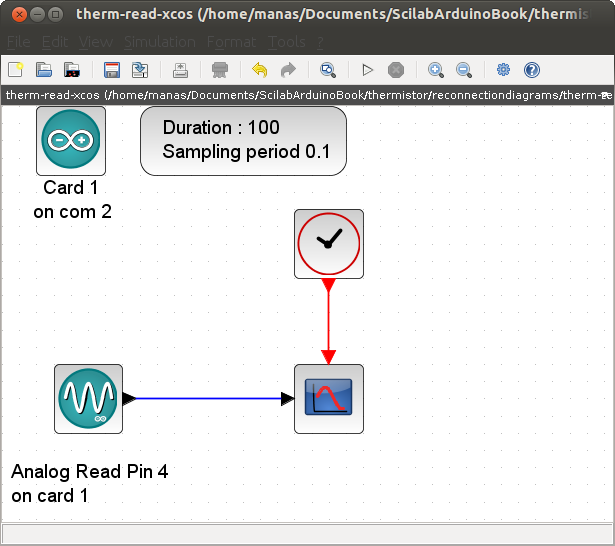
\includegraphics[width=\smfigp]{\LocTHERMfig/therm-read-xcos.png}
    \caption[Xcos diagram to read thermistor values]{Xcos diagram to
      read thermistor values.  This is what one sees when
      \LocTHERMscibrief{therm-read-xcos.zcos}, is invoked.}
    \label{fig:therm-read}
  \end{figure}
  The parameters of the blocks can be changed by right clicking on the
  block and choosing {\tt Block Parameters}. One can also double click
  on the block. The values for each block is tabulated in
  \tabref{tab:therm-read}.  All other parameters are to be left
  unchanged.

  \begin{table}
    \centering
    \caption{Xcos parameters to read thermistor}
    \label{tab:therm-read}
    \begin{tabular}{llc} \hline
      Name of the block & Parameter name & Value \\ \hline
      ARDUINO\_SETUP & Identifier of Arduino Card & 1 \\
      & Serial com port number & 2\portcmd \\ \hline
      TIME\_SAMPLE & Duration of acquisition(s) & 100 \\
      & Sampling period(s) & 0.1 \\ \hline
      ANALOG\_READ\_SB & Analog Pin & 4 \\
      & Arduino card number & 1 \\ \hline
      CSCOPE & Ymin & 200 \\ 
      & Ymax & 600 \\
      & Refresh period & 100 \\ \hline
      CLOCK\_c & Period & 0.1 \\
      & Initialisation Time & 0 \\ \hline
    \end{tabular}
  \end{table}
  \begin{figure}
    \centering
    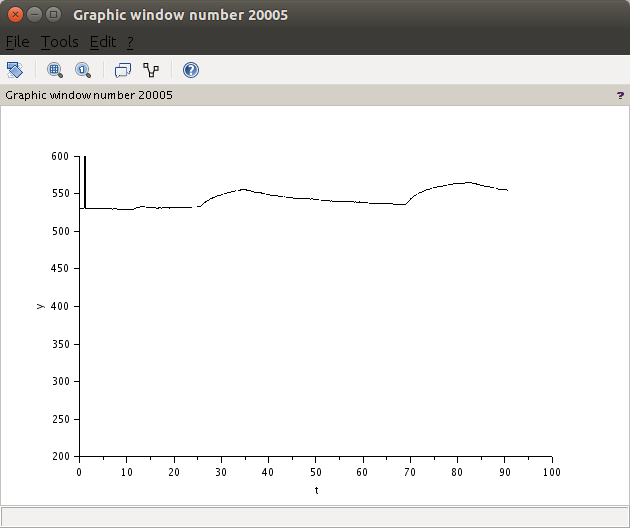
\includegraphics[width=\smfigp]{\LocTHERMfig/therm-read.png}
    \caption[Output of Xcos diagram to read thermistor values]{Output
      of Xcos diagram to read thermistor values.  This is what one
      sees when \LocTHERMscibrief{therm-read-xcos.zcos}, is executed.}
    \label{fig:therm-read-output}
  \end{figure}
  The thermistor readings can be varied by bringing a heating or
  cooling source in the vicinity of it. The graph as shown in
  \figref{fig:therm-read-output} will show the variations in the ADC
  output that is displayed.

\item In the second experiment, we will switch On and Off a buzzer
  depending on the thermistor readings (ADC output). The xcos diagram
  for this experiment is as shown in \figref{fig:therm-buzzer}.
  \begin{figure}
    \centering
    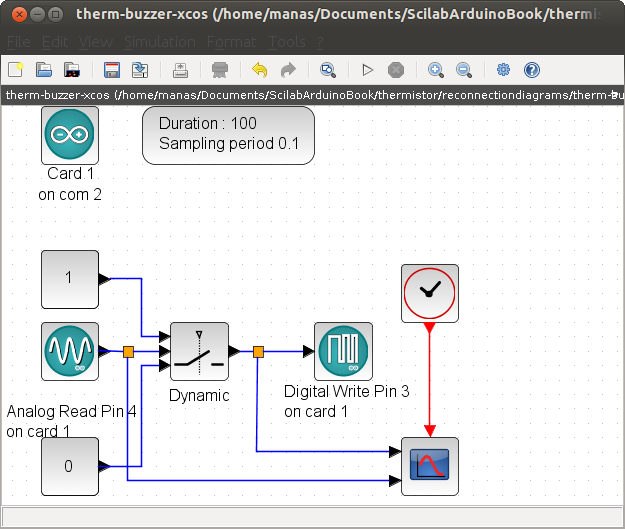
\includegraphics[width=\lgfig]{\LocTHERMfig/therm-buzzer-xcos.png}
    \caption[Xcos diagram to read the value of thermistor, which is
    used to turn the buzzer on or off] {Xcos diagram to read the value
      of the thermistor, which is used to turn the buzzer on or off.
      This is what one sees when
      \LocTHERMscibrief{therm-buzzer-xcos.zcos}, is invoked.}
    \label{fig:therm-buzzer}
  \end{figure}
  The parameters of the blocks can be changed by right clicking on the
  block and choosing {\tt Block Parameters}. One can also double click
  on the block. The values for each block is tabulated in
  \tabref{tab:therm-read}.  All other parameters are to be left
  unchanged.

\begin{table}
    \centering
    \caption{Xcos parameters to read thermistor and switch the buzzer}
    \label{tab:ldr-led}
    \begin{tabular}{llc} \hline
      Name of the block & Parameter name & Value \\ \hline
      ARDUINO\_SETUP & Identifier of Arduino Card & 1 \\
      & Serial com port number & 2\portcmd \\ \hline
      TIME\_SAMPLE & Duration of acquisition(s) & 100 \\
      & Sampling period(s) & 0.1 \\ \hline
      ANALOG\_READ\_SB & Analog pin & 4 \\
      & Arduino card number & 1 \\ \hline
      CMSCOPE & Ymin & 0 300 \\ 
      & Ymax & 1 600 \\
      & Refresh period & 100 100 \\ \hline
      CLOCK\_c & Period & 0.1 \\
      & Initialisation time & 0 \\ \hline
      SWITCH2\_m & Datatype & 1 \\
      & threshold & 550 \\
      & pass first input if field & 0 \\
      & use zero crossing & 1 \\ \hline
      DIGITAL\_WRITE\_SB & Digital pin & 3 \\
      & Arduino card number & 1 \\ \hline
    \end{tabular}
  \end{table}
  The graph as shown in \figref{fig:therm-buzzer-output} will show the
  variations in the ADC output that is displayed and the corresponding
  switching of buzzer whenever the limits are crossed.
  \begin{figure}
    \centering
    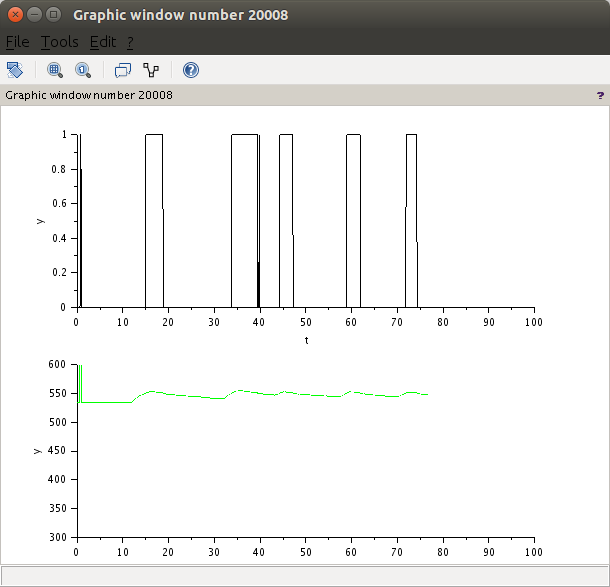
\includegraphics[width=\smfig]{\LocTHERMfig/therm-buzzer.png}
    \caption[Output of Xcos diagram to switch buzzer through
    thermistor values]{Output of Xcos diagram to switch buzzer through
      thermistor values. This is what one sees when
      \LocTHERMscibrief{therm-buzzer-xcos.zcos}, is executed.}
    \label{fig:therm-buzzer-output}
  \end{figure}
\end{enumerate}

\section{Interfacing the Thermistor from Python}
\subsection{Interfacing the Thermistor}
In this section we will explain a few python scripts to read values
from thermistor and to use them.  The {\tt cmd\_analog\_in} command
will be used to read from thermistor connected to an analog input
pin. The experiments will be carried out using python.

\begin{enumerate}
\item In the first experiment, \pyref{py:therm-read} is used to read
  values from thermistor. First the serial port is opened using the
  command {\tt open\_serial} and passing the correct port number to
  it. The command {\tt cmd\_analog\_in} is used to read from the
  analog pin. The pin number is passed to this command as an
  argument. The read value is stored in some variable. The value is
  then displayed on the scilab console. A sleep of 500 millisecond is
  executed using the {\tt sleep} command and then the reading process
  is repeated 20 times by putting it in a {\tt for} loop. After the
  loop is finished the serial port is closed using the {\tt
    close\_serial} command.

\item In the second experiment, we will use the python script to
  turn a buzzer on and off using the thermistor values. The changes in
  the thermistor resistance is sensed as a voltage change between 0 to
  5V. The ADC maps the thermistor voltage readings in to values
  ranging from 0 to 1023. This means 0 for 0 volts and 1023 for 5
  volts. In this experiment we compare the ADC output value with 550
  and as soon as the value exceeds 550 the buzzer is turned on. See
  \sciref{py:therm-buzzer} for the complete code. We use {\tt if}
  loop to achieve this functionality. Command {\tt cmd\_digital\_out}
  is used to turn the buzzer on and off.  The correct port number on
  which the buzzer is connected is passed to this command as an
  argument. The entire process is repeated 500 times.
\end{enumerate}

\subsection{Python Code}
\label{sec:therm-pyhton-code}
\addtocontents{pyd}{\protect\addvspace{\codclr}}

\begin{pycode}
  \pcaption{Read and display the thermistor values} {Read and display
    the thermistor values.  Available at
    \LocTHERMpybrief{therm-read.py}.}
\label{py:therm-read}
\lstinputlisting{\LocTHERMpycode/therm-read.py}
\end{pycode}

\begin{pycode}
  \pcaption{Turning the buzzer on and off using thermistor values}
  {Turning the buzzer on and off using the thermistor values read by
    ADC.  Available at \LocTHERMpybrief{therm-buzzer.py}.}
\label{py:therm-buzzer}
\lstinputlisting{\LocTHERMpycode/therm-buzzer.py}
\end{pycode}

\section{Interfacing the Thermistor from Julia}
\subsection{Interfacing the Thermistor}
In this section we will explain a few julia scripts to read values
from thermistor and to use them.  The {\tt analogRead} command
will be used to read from thermistor connected to an analog input
pin. The experiments will be carried out using python.

\begin{enumerate}
\item In the first experiment, \juliaref{julia:therm-read} is used to read
  values from thermistor. First the serial port is opened using the
  command {\tt connectBoard}. The command {\tt analogRead} is used to read from the
  analog pin. The pin number is passed to this command as an
  argument. The read value is stored in some variable. The value is
  then displayed on the Atoms console. A sleep of 500 millisecond is
  executed using the {\tt sleep} command and then the reading process
  is repeated 20 times by putting it in a {\tt for} loop. After the
  loop is finished the serial port is closed using the {\tt
    close } command.

\item In the second experiment, we will use the julia script to
  turn a buzzer on and off using the thermistor values.The whole
  process is same as described in the python code. 
\end{enumerate}

\subsection{Julia Code}
\label{sec:therm-julia-code}
\addtocontents{juliad}{\protect\addvspace{\codclr}}

\begin{juliacode}
\jcaption{Read and display the thermistor values} {Read and display
    the thermistor values.  Available at
  \LocTHERMjuliabrief{therm-read.jl}.}
\label{julia:therm-read}
\lstinputlisting{\LocTHERMjuliacode/therm-read.jl}
\end{juliacode}

\begin{juliacode}
\jcaption{Turning the buzzer on and off using thermistor values}
  {Turning the buzzer on and off using the thermistor values read by
    ADC.  Available at \LocTHERMjuliabrief{therm-buzzer.jl}.}
\label{julia:therm-buzzer}
\lstinputlisting{\LocTHERMjuliacode/therm-buzzer.jl}
\end{juliacode}

\section{Interfacing the Thermistor from OpenModelica}
\subsection{Interfacing the Thermistor}
In this section we will explain a few OpenModelica scripts to read values
from thermistor and to use them.  The {\tt cmd\_analog\_in} command
will be used to read from thermistor connected to an analog input
pin. The experiments will be carried out using OpenModelica.

\begin{enumerate}
\item In the first experiment, \OpenModelicaref{OpenModelica:therm-read} is used to read
  values from thermistor. First the serial port is opened using the
  command {\tt open\_serial} and passing the correct port number to
  it. The command {\tt cmd\_analog\_in} is used to read from the
  analog pin. The pin number is passed to this command as an
  argument. The read value is stored in some variable. The value is
  then displayed on the OpenModelica ourput console. A delay of 500 millisecond is
  executed using the {\tt delay} command and then the reading process
  is repeated 20 times by putting it in a {\tt for} loop. After the
  loop is finished the serial port is closed using the {\tt
    close\_serial} command.

\item In the second experiment, we will use the OpenModelica script to
  turn a buzzer on and off using the thermistor values. The changes in
  the thermistor resistance is sensed as a voltage change between 0 to
  5V. The ADC maps the thermistor voltage readings in to values
  ranging from 0 to 1023. This means 0 for 0 volts and 1023 for 5
  volts. In this experiment we compare the ADC output value with 550
  and as soon as the value exceeds 500 the buzzer is turned on. See
  \OpenModelicaref{OpenModelica:therm-buzzer} for the complete code. We use {\tt if}
  loop to achieve this functionality. Command {\tt cmd\_digital\_out}
  is used to turn the buzzer on and off.  The correct port number on
  which the buzzer is connected is passed to this command as an
  argument. The entire process is repeated 500 times.
\end{enumerate}

\subsection{OpenModelica Code}
\label{sec:therm-OpenModelica-code}
\addtocontents{OpenModelicad}{\protect\addvspace{\codclr}}

\begin{OpenModelicacode}
\mcaption{Read and display the thermistor values} {Read and display
    the thermistor values.  Available at
  \LocTHERMOpenModelicabrief{therm-read.mo}.}
\label{OpenModelica:therm-read}
\lstinputlisting{\LocTHERMOpenModelicacode/therm-read.mo}
\end{OpenModelicacode}

\begin{OpenModelicacode}
\mcaption{Turning the buzzer on and off using thermistor values}
  {Turning the buzzer on and off using the thermistor values read by
    ADC.  Available at \LocTHERMOpenModelicabrief{therm-buzzer.mo}.}
\label{OpenModelica:therm-buzzer}
\lstinputlisting{\LocTHERMOpenModelicacode/therm-buzzer.mo}
\end{OpenModelicacode}
